%!TEX root = ../main.tex
\chapter{An Unified Efficient Particle Physics Framework}
\label{new_lipmini}

Developing parallel code for heterogeneous platforms is more complex than for homogeneous platforms. In a shared memory context, the data is always accessible by the programmer, as the different memory bank accesses on multi-CPU systems are managed by the compiler and hardware. Data dependencies and concurrent memory accesses still need to be managed by the programmer, which may required a significant level of expertise. To efficiently use the computational resources, dealing with problems such as false sharing and efficient cache usage, the programmer must have an advanced expertise on both the coding and architectural knowledge of homogeneous platforms.

Heterogeneous platforms are organised in a distributed memory environment, where the CPUs share the memory among each other but not with the hardware accelerators, which rises a new set of challenges. All communications of data between CPU and accelerator must be explicitly coded by the programmer, and has an added latency associated. The balance of the workload for each computing device to process becomes harder as it must take into account the data transfers and different characteristics of the devices.

Each different hardware accelerator has its own architectural design principles, as presented in section \ref{hardware}, which constrain their programming paradigm and the characteristics that both the algorithm and the code must have to efficiently use the computational resources. This implies that the programmer must be able to learn the hardware intrinsic characteristics and adapt to a new programming paradigm. Even for experienced programmers, porting current applications to run on heterogeneous platforms may be infeasible without redesigning the core features, which does not happen when designing a new application from scratch specifically for these platforms. Legacy code suffers the most from these issues.

Scientists are usually self-taught programmers that only develop applications as they are a necessary tool for the research in their field. Several studies, referred in section \ref{goals}, identified a set of problems with the scientists coding practices and scientific computing. Most of their code is in constant development, which may last for decades, adding and changing functionalities in each development iteration, disregarding most software engineering principles and not adapting the code to the hardware evolution. The few scientists that worry about performance attempt to optimise the code regions that they think are the bottleneck, not knowing of the existence of profiling tools.

Since most scientists develop applications with the help of specialised frameworks of their research field, they expect that the tools coded efficiently and use the multicore capabilities of modern CPUs. However, the bottleneck is often on the developed code rather than in the framework, and these tools are not designed to automatically parallelize the bottlenecks and balance the workload among the available computing units.

Scientists opt to spend most of the research time on studying the problem and enhancing the algorithms rather than improving their programming skills to efficiently use the platforms available on modern computing clusters. They are even more reluctant to learn the new programming paradigms required to code for hardware accelerators on heterogeneous platforms. Several automatically parallelization and load balancing frameworks were developed for these systems by computer scientists to help the scientific community, as presented in subsection \ref{distributed_mem}.

These general purpose frameworks usually have a steep learning curve, even for computer scientists. One significant setback of these frameworks is that, even if it is not explicitly required, the application must be designed to the framework characteristics, rather than the framework adapt to the application. As scientists are usually reluctant to redesign the very complex legacy code, which is difficult for computer scientists to understand without the expertise of the science field, an integration with these frameworks is infeasible. This problem also applies to the most of the external libraries used by these applications, as their functions are not coded to run on hardware accelerators and adapting the source code may not be possible.

Scientists are not willing to endure the steep learning curve of these frameworks to integrate with the development of future applications, and, as required by some frameworks, do not want to code two versions of an algorithm to run on the CPU and accelerator. The architectural complexity of these systems and the lack of guarantees to that the code performance will improve, due to poor implementation or algorithm characteristics, drives the scientists away from these frameworks. Finally, scientists attempt to produce applications with few external libraries dependencies, as they are not guaranteed to be supported through the application lifetime.

The existence of general purpose load balancing frameworks for heterogeneous platforms is useful, specially for computer scientists, but the scientific community lacks frameworks that both address the intrinsics of their scientific field, in which scientists can trust and rely, and the efficient usage of the computational resources, on both homogeneous and heterogeneous platforms. Frameworks such as these sacrifice the abstraction required to interact with any scientific field, but are more adapted to the addressed scientific problem. A more concise framework orientation leads to an easy interaction of the scientist with the tool (and better abstraction of the parallelization complexities) and increases the computational efficiency of the code, when compared with general purpose frameworks. The main bottlenecks are usually known \textit{a priori} and the framework is designed around the problem characteristics. The development of such frameworks may lead to a better interface between computer scientists and other scientific researchers, which may improve their codes and increase the quality of the research.

\section{The LipMiniAnalysis Skeleton Library}
\label{lipminianalysis}

The LipCbrAnalysis was a skeleton developed by two researchers of LIP in 2005, with the purpose of aiding the development of data analysis applications within the research group. Initially it served as an interface for dealing with the I/O of the data, transforming the input data ROOT format to variables in the global memory of the skeleton. Function prototypes for the features common among data analysis applications were declared on the skeleton. The programmer would code the functions to each analysis specific needs, knowing that all data was addressable from a global context.

Along the years the code was successively iterated to add support for new data file formats, physics functionalities, and general features, such as the support for passing options and arguments to the executable. Some of the functions that the programmer needed to code were now fully implemented, with the option of being override by the user.

The LipMiniAnalysis is the latest development iteration of LipCbrAnalysis currently on production. It discarded features that were no longer necessary, and was adapted to read the new Mini Ntuple data format, hence its name. It is not a standard ROOT format, but results from a refinement and partial filtering of the events to improve the data quality.

Figure \ref{fig:lipmini} presents the structure of LipMiniAnalysis, where all orange sections need to be coded by the programmer. When the application starts it sets the default values for all control information needed by the event filtering and reconstruction. The \textit{Set User Values} section allows for the user to set its own control parameters, for both information defined by \textit{Set Default Values}, overwriting the existing configuration, and other parameters not yet set. The \textit{Get Command Line Options} section is responsible for defining and interpreting the options defined by the user when starting the executable. It is partially defined with standard options for every analysis, such as the definition of the systematics file and output directory, but the programmer can add new options as needed. The systematics parameters are automatically configured based on the input systematics file, and no user interaction is necessary. The preparation of both the input and output files is done automatically, but the declaration of the histogram vectors must be coded by the programmer, as it depends on the event type, filtering and reconstruction techniques applied.

\begin{figure}[!htp]
	\begin{center}
		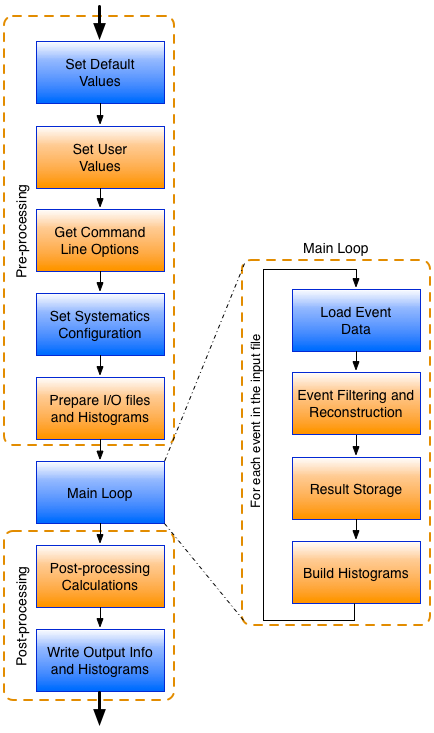
\includegraphics[scale=0.5]{imgs/lipminianalysis.png}
		\caption{Schematic representation of the LipMiniAnalysis skeleton structure. The programmer is required to code the orange sections of the flow.}
		\label{fig:lipmini}
	\end{center}
\end{figure}

The \textit{Main Loop} has a loop over all events on the input data file that loads a single event, applies the filters, reconstructs the event it if it passes the required filters, stores the results, and builds the histograms for each filter and final reconstruction. Only the event loading is automatic, so the programmer is required to code all remaining sections, as they vary among different analysis. The final post-processing also depends on the analysis. Then, LipMiniAnalysis automatically writes all output information. Note that this is a logical structure of the code; in the current implementation most features are not properly organised and LipMiniAnalysis would have great benefits from a reorganisation of its code.

Studies presented in \cite{Msc:AMP,paperAMP} targeted the computational efficiency issues of a specific data analysis application of LIP, related to the reconstruction of the \ttH system. This data analysis was developed using the LipMiniAnalysis and, although the goal of the work was to address only the inefficiencies of the data analysis itself, problems with the main data structure of the skeleton library restricted the performance scalability, specially on heterogeneous platforms.

The LipMiniAnalysis was designed to store only one event in the application global memory for the \textit{Main Loop} to load and process. The data for an event is composed of hundreds of variables, ranging from simple scalars to complex vectors of ROOT classes. With only a single event in memory, it is more difficult to create an efficient parallelization with only the event reconstruction tasks, due to the low amount of work to balance, specially on distributed memory environments as it will require more communications in the application runtime. The filtering of events cannot be performed in parallel as the filters have data dependencies among them. With all events from an input data file on the application global memory, a more efficient parallelization for both shared and distributed memory systems can be achieved. It would also help the implementation of automatic parallelization and load balancing in LipMiniAnalysis.

\section{The Proposed Framework for Particle Physicists}
\label{new_framework}

A physics framework is proposed to replace LipMiniAnalysis in aiding the development of data analysis applications. Its design and specification will include several software engineering concepts to provide a stable and robust tool that will increase the researchers productivity, spending less time coding and more time analysing data and improving physics algorithms. It will ensure the generation of efficient data analysis applications by providing automatic parallelization and load balancing mechanisms. It will include both redesigned features of LipMiniAnalysis and new particle physics functionalities.

Improving both the researchers coding productivity and data analysis computational efficiency has a direct impact on the research quality. To achieve this goal, the proposed framework has to utilise the capabilities of modern computing systems and software. This implies that the LipMiniAnalysis code design, based on the LipCbrAnalysis developed in 2005, cannot be used as it does not fit the characteristics of modern hardware. The new framework will implement all required features present in LipMiniAnalysis but designed to modern hardware specifications.

Figure \ref{fig:new_framework} presents the organisation and dependencies of the different modules of the proposed framework. A modular organisation and implementation allows for the framework to be robust and easily extensible in the future. The \textit{Physics} and \textit{Histograming} modules will be implemented using redesigned features currently available at LipMiniAnalysis, as they are used by most data analysis applications. The framework will have to support both ROOT and TopROOTCore libraries without requiring any specific configuration by the user. TopROOTCore installation with the framework may be an option to the user, since only a subset of data analysis applications use its functionalities.

\begin{figure}[!htp]
	\begin{center}
		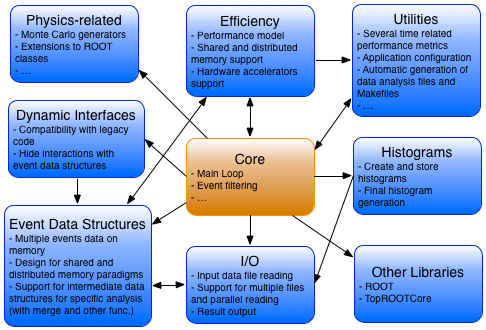
\includegraphics[scale=0.7]{imgs/new_framework.png}
		\caption{Schematic representation of the proposed framework modules and their dependencies.}
		\label{fig:new_framework}
	\end{center}
\end{figure}

The \textit{I/O} module is responsible for loading the input data files for processing the events. The LipMiniAnalysis reads only MiniNtuples, which are preprocessed events at the previous computational tiers, used by some applications, but other file formats will also be supported, after analysing the current formats used by researchers. Different file formats have different structures and auxiliary parameters, although the core event information is similar. The file reading must support parallel file descriptors, so that it is possible that each thread/process reads its own event data, reducing the communications cost and initial load distribution overhead. Since the size of an input data file is around 1 GBytes, the framework will support a batch of input files and will manage their execution.

The \textit{Event Data Structures} module will be dependent on the file type to be read. Its purpose is to have a C++ class, or set of classes, to hold all the information of an event on memory in a structured way, opposed to the current implementation on LipMiniAnalysis. The module will use a collection (vector, map, etc) to store the instantiations of the event class, enclosing all events in one or multiple input data files. An assessment of the different file formats used at LIP will be required to evaluated the benefits of having a single abstract event class or specific classes for each file format. Both the event class design and store collection must be suitable for both shared and distributed memory parallelization, with good performance on data structure splits (to balance the load, specifically in distributed memory paradigms), transverses (to iterate through the events on each split segment), and low overhead on (un)marshalling computations for communicating the data among processes. The module may also contain specific data structures for intermediate processing, as explained in detail in subsection \ref{work_so_far}, suitable to run on hardware accelerators.

The \textit{Dynamic Interfaces} module will hold the interface generator and respective interfaces for each different event data structure. Its purpose is to make the framework compatible with legacy code, allowing for current data analysis applications to benefit from the automatic parallelization and improved efficiency of the proposed framework. Also, it must hide the interaction of the user with the data structures, to provide a simpler programming interface, which is explained in more detail in subsection \ref{usage_workflow}. Since there may be several different data structures, and their code may be changed periodically, the interface generator must be capable of parsing the data structure source files and generate the interfaces at compile time.

The \textit{Utilities} module implements several auxiliary features usable in both the framework and data analysis code. It will have simple performance statistics, such as execution time of the application, communications time, event processing throughput, etc. A more robust command line options reader will be available, with all required options for executing all different data analysis, which can be extended by experienced users.

The \textit{Efficiency} module will have all necessary functionality required to create parallel tasks and manage the load distribution for both homogeneous and heterogeneous platforms with hardware accelerators. The performance model must be capable of assessing if an hybrid thread/process parallelization provides better efficiency than a simple multithreaded implementation, which was proven to happen in some data analysis \cite{paperAMP}. There is no automatic parallelization tool that attempts hybrid implementations such as this, only opting for a shared or distributed memory paradigm (usually the last is only used when the hardware forces to), but it may prove beneficial to have this mix of processes and threads in some specific cases. This may require more time to obtain the best process/thread configuration, but since these data analysis run for several hours the initial overhead is minimum. It also can produce a configuration file when the setup is performed for a given data analysis on a given computing system to avoid executing the initial setup every time the application starts.

This module must also be able to assess, possibly with some help of the user, which sections of the data analysis code can be executed in the hardware accelerators, and if they have the required characteristics to efficiently use these devices. While this might seem complex for general purpose parallelization frameworks, dealing with only a specific problem of particle physics data analysis applications helps to design and adapt the performance model around this field features. A new framework implementation designed to this specific problem, with components adapted from current frameworks, may provide a better and simpler integration, and improve the efficiency of data analysis applications, which would not be possible by using existing libraries.

The \textit{Core} module will integrate all previous modules, implementing the major routines responsible for the event analysis, ranging from the filtering to the final output data storage. It assembles all the specific bits of each module to process the events, as well as the code sections that are for the user to code. Note that the user will not edit the code in the framework, but rather create a data analysis source file that will link to the framework.

Relevant features for most compute intensive sections of data analysis applications will be implemented to run on CPU and accelerator devices and will be provided in the framework API. For example, when selecting an pseudo-random number generator to use in a compute intensive section, such as the event reconstruction, the user must avoid the \texttt{TRandom} available in ROOT and use the one provided by the framework. The framework compiles the code to run on CPU, which uses \texttt{TRandom}, and on GPU, which may use the \texttt{cuRand} (with the same PRNG algorithm). This only applies for features that produce the same result on any computing accelerator. Otherwise, an alternative is suggested for each computing device that the user may chose to accept.

\subsection{Usage and Workflow}
\label{usage_workflow}

One of the goals of the framework is to provide a kernel-like programming model to the user, abstracting most parallel programming complexities. This eases the development of new data analysis applications and increases their portability across platforms. Its flow is presented in figure \ref{fig:new_framework_flow}. Note that LipMiniAnalysis, presented in section \ref{lipminianalysis}, has a similar logical structure, but it does not reflect the code organisation and structure. In the new framework, the code will follow this structure to improve its modularity and reliability.

\begin{figure}[!htp]
	\begin{center}
		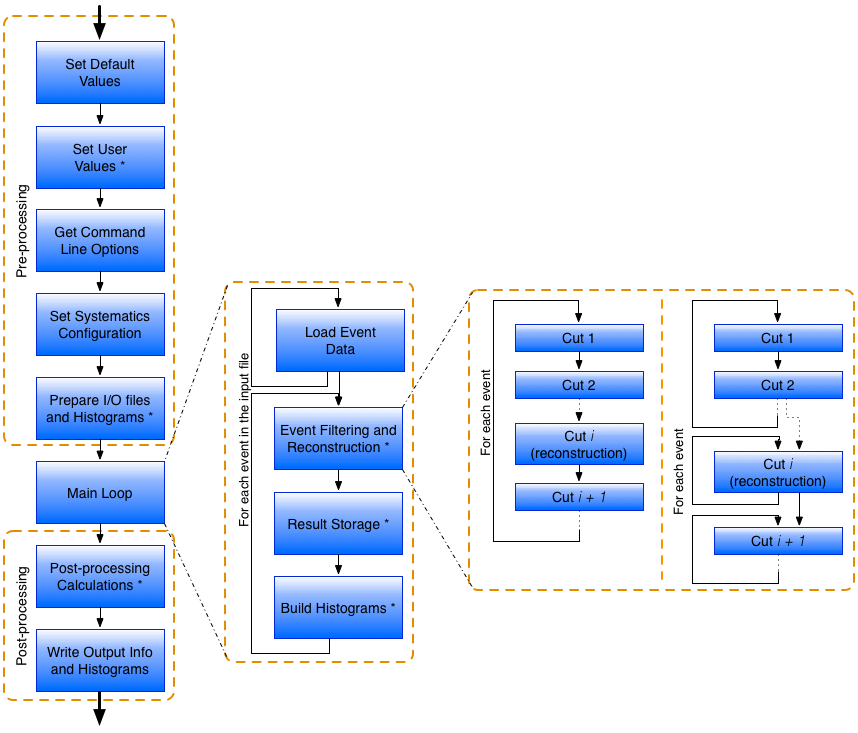
\includegraphics[scale=0.5]{imgs/new_framework_flow.png}
		\caption{Schematic representation of the proposed framework flow. The programmer must code the orange sections of the flow.}
		\label{fig:new_framework_flow}
	\end{center}
\end{figure}

The user intervention is required at four stages of the event processing (implementation-wise, the \textit{Result Storage} and \textit{Build Histograms} are coded together as \textit{Filter Post-process}). The data analysis is expected to be implemented as a class, which will extend the \texttt{DataAnalysis} class provided by the framework, and must contain a set of predefined methods that represent each of the stages. The user codes the filters and reconstruction for a single event assuming that the data is on global memory. The user does not interact directly with the event data structure, but through the respective interface, which gives the illusion that only a single event is on memory, as physicists were used to program so far. The framework will be responsible for applying the code in parallel to all events on memory, not necessarily following the pipeline order but respecting the dependencies.

The data analysis stages are characterised as follows:

\begin{description}
	\item[\textit{User Setup}:] this is only executed at the beginning of the data analysis execution, where the user specifies the initial \textit{User Values}, as in the LipMiniAnalysis flow, output files, and histogram configurations. Expert users can also specify any additional parameters to read by both command line and environment variables, using the respective framework utilities, and a small set of configurations to help the parallelization setup.
	\item[\textit{Event Filtering and Reconstruction}:] this section filters and reconstructs a single event. As shown in figure \ref{fig:new_framework_flow}, two templates are provided. The first is the traditional pipeline for the event processing, oriented for novice users. The second provides three sections: pre-filtering, reconstruction, and post-filtering. The user codes in the pre-filtering the filters applied before the reconstruction, the reconstruction, and then the final filters (if applicable), in three separate methods. This is useful when the reconstruction takes most of the execution time as it allows for better load balance, specially when the framework can use accelerators for the reconstruction.
	\item[\textit{Result Storage} and \textit{Build Histograms}:] this is coded as a single method, since both operations are closely dependent in most implementations. The user store the results of the previous filtering to later be printed in the output file.
	\item[\textit{Post-processing Calculations}:] this stage is executed once, after processing all events. The user codes all final calculations before the results and histograms output.
\end{description}

The design of the stages required by the \texttt{DataAnalysis} class will be refined after the requirements elicitation and an usability study with the LIP researchers. All major features initial design and testing was performed in close cooperation with a subset of LIP physicists, working on top quark and Higgs boson research.

The programmer will have some guidelines to avoid producing an inefficient data analysis. Class variables in \texttt{DataAnalysis} must be avoided because of the amount of communications required to maintain the consistency and coherence of that data on a distributed memory environment. To maintain portability, the data analysis must only depend on the libraries provided by the framework (at the moment, there is not any data analysis in LIP that depends on other libraries). To run on heterogeneous platforms, the analysis critical region must only depend on features that the framework has implemented for both CPU and accelerator devices. This allow the user to code the section so that it is able to execute on any computing device. Otherwise, the code will be restricted to the device that can compute it.

\subsection{Preliminary Prototypes}
\label{work_so_far}

Some features of the framework modules were developed. These prototypes were integrated and tested with the current version of LipMiniAnalysis, using the \ttH data analysis application presented in section \ref{particle_frameworks}, but have a modular design to be properly merged into the final framework. The proposed prototypes of these features are presented next.

\subsubsection*{A new event data structure}

The information of an event is loaded in the \textit{Main Loop} into a single global memory state. The hundreds of variables of an event are spread among a set of files of LipMiniAnalysis. To create a new event data structure all these variables were merged into a single C++ class, which represents a single event, named \textit{EventData}, and use a standard collection, such as a STL vector, was used to store all events of an input file. However, the current LipMiniAnalysis version performs a set of data preparation routines, named \textit{FillAllVectors} and \textit{Calculations} (the latter needs to be coded by the user). As their implementation is only prepared to access the data as it was in the global memory, they will not be compatible with the new data structure. 

The implementation of \textit{Calculations} could be changed in order to access the values stored in the new data structure. However, the user would have to be aware of the data structure interaction and characteristics to properly code the required data preparation. Since \textit{Calculations} only accesses the data of an event, it makes much more sense to code it as a method of the event class. The current implementation of \textit{EventData}, the \textit{FillAllVectors} routine, which performs the initialisation of some of the components of an event, is coded as a method, and the \textit{Calculations} is declared as a virtual function, so it can be coded by the user in the analysis source file, without the need to interact with LipMiniAnalysis.

\subsubsection*{A new \textit{Main Loop} design}

Having a new data structure that allows multiple events to be on memory simultaneously implies changes to the way that LipMiniAnalysis handles the input data files. Instead of loading an event at a time, the \textit{Main Loop} implementation was changed to load all events in an input data file at once, and store them in the new specialised structure, as presented in figure \ref{fig:new_loop}. Now, it is possible to parallelize the execution of the \textit{Event Filtering and Reconstruction}, performed in the \textit{DoCuts} function. In physics terminology, a filter is addressed as a cut.

\begin{figure}[!htp]
	\begin{center}
		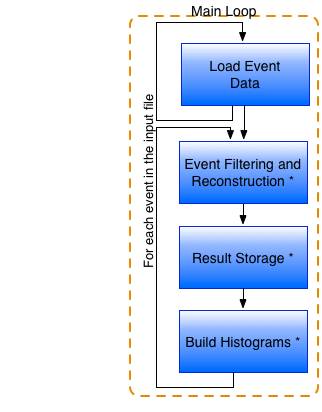
\includegraphics[scale=0.5]{imgs/new_loop.png}
		\caption{Schematic representation of the new \textit{Main Loop} implementation.}
		\label{fig:new_loop}
	\end{center}
\end{figure}

The interaction of the LipMiniAnalysis with the input data file is performed using the ROOT file reader classes. Since the event loading assumes a set of operations, such as storing MonteCarlo information on \textit{EventData} and the \textit{FillAllVectors} initialisation, this task would benefit if it was executed in parallel, as the I/O itself only amounts to a small part of the computation. However, up to version ROOT v6, released in early June, it was not possible to have parallel file descriptors reading information of the same input file. With the new ROOT version it may be possible but it was not yet tested.

The purpose of the filters is to separate the signal (interesting events) from the background (uninteresting events). This notion depends on the physics that the analysis studies as, for example, the background of a \ttH system analysis may contain events useful for the search of heavy quarks. As it may vary among different analysis, the \textit{DoCuts} must be coded by the user, but its structure is well defined. Implementation-wise, an analysis has a set of filters. Each filter is logically composed by a set of computations, more or less complex, and a test to the results of those computations. If the test fails, the event is discarded. An example of a simple filter is to check if the mass of the event system (aggregate masses of all or a subset of particles detected) is greater than a given value.

The reconstruction of an event is considered a filter in \textit{DoCuts}, as only the events capable of being reconstructed pass the filter, and is usually the last. The reconstruction is usually the most complex and computational intensive task in the whole data analysis application. One example is the \ttH system reconstruction, which performance depends on a trade-off between reconstruction accuracy and execution time. The event reconstruction is a task that may require a closer analysis to improve the efficiency of the application, through a more specific parallelization on both homogeneous and heterogeneous platforms. Its irregular workload, very complex algorithms, and few vectorised numerical computations create a complex bottleneck, but has the potential of greatly improving the performance when properly optimised \cite{paperAMP}. Figure \ref{fig:new_docuts} presents the implemented prototype for a new \textit{DoCuts} flow that exposes the event reconstruction to more efficient parallelization mechanisms.

\begin{figure}[!htp]
	\begin{center}
		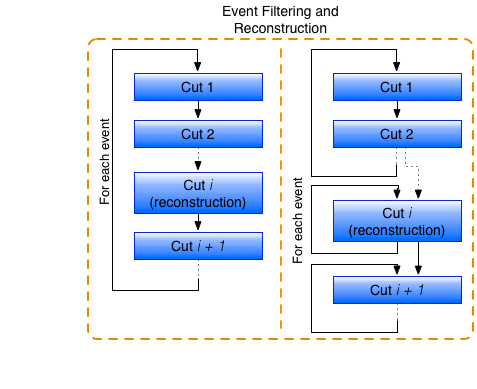
\includegraphics[scale=0.5]{imgs/new_docuts.png}
		\caption{Schematic representation current (left image) and proposed (right image) \textit{Event Filtering and Reconstruction} flows.}
		\label{fig:new_docuts}
	\end{center}
\end{figure}


Besides exposing the parallelism of a complex computational intensity section, this change also increases the events to be simultaneously reconstructed. When the application reaches the reconstruction, all events that passed the previous cuts can be processed in parallel. Having all the data necessary outside of the \textit{Main Loop} loop allows for a better load balance of the possible parallelization approaches using hardware accelerators. It also helps to reduce the parallelization overhead associated with the communications in heterogeneous systems: instead of passing required the data of a single event multiple times, the data of all events is passed once. There is a third section of cuts (post-reconstruction) that are also coded by the user. To reduce the amount of loops, this third section shares the loop over all events with all the remaining post-processing of the \textit{Main Loop}. Note that both \textit{Main Loop} options will be available to maintain compatibility with the legacy data analysis applications.

\subsubsection*{Interfacing with legacy code}

Current data analysis use the data of an event as it is on the global memory, with no structure. The integration of the new event data structure requires that the accesses to the data be made through the STL collection used to store the event and the \textit{EventData} class. An interface is proposed to avoid rewriting the legacy code of these data analysis, providing a kernel-like programming approach (where the code for processing an event is applied to all simultaneously). The interface must abstract the access to both the \textit{EventData} variables and methods.

The input data file format occasionally suffers some changes due to the increase in information given by the previous preprocessing on the CERN computational tiers. The file reading and the \textit{EventData} classes have to be adapted to this increase in event parameters. A static interface would need to be rewritten every time such change occurred. A parser was developed to solve this problem by receiving the \textit{EventData} source files and retrieving the name of the methods and parameters. It then creates a header composed of \textit{define} clauses that translate the accesses to these variables on the STL collection to simple global accesses. This header is then included in the main LipMiniAnalysis so that the user does not need to interact with the interface. This interface is automatically created every time the skeleton is compiled.

With this, the user can code the data analysis assuming a single event is stored in memory. For example, to access an event luminosity the user would write \texttt{int var = LumiBlock}. However, when compiling the application the compiler preprocessor uses the interface to replace that statement with \texttt{int var = events.get(currentEvent).getLumiBlock()}, without the user knowing how the event is stored. The framework manages the counter that assigns the event to process in every loop that iterates through the event data structure.

\subsubsection*{Other features}

The framework will have an utility module where general features will be included. Some of the already implemented range from automatic execution time measurement of the application and event processing throughput, definition of the number threads to execute, and setting the accuracy of some reconstructions. It was opted to use environment variables to set these features to reduce the clutter of options currently passed to the data analysis applications (usually more than 10 parameters) and separate general purpose features from physics functionalities.

One complex feature was implemented specifically for the \ttH data analysis application. During the event reconstruction, several different variations of the system are reconstructed and only the best is of interest. For that a class was developed that encloses the resultant data of the reconstruction and performs a parallel merge through all the threads. This feature might prove useful for other data analysis once the structure of the class is general enough to hold the result of different types of reconstructions.

\subsection{The Underlying Middleware for Heterogeneous Environments}
\label{middleware}

Subsection \ref{distributed_mem} presents various libraries for efficient load balancing in heterogeneous platforms. The most relevant are DICE, StarPU, and Legion, which provide efficient parallelization and load balance mechanisms for irregular workloads, but only support GPU hardware accelerators. Since these libraries are target for users with expertise in parallel programming for heterogeneous platforms, and they require that the applications to be developed according to their specifications, they are not usually adopted by non-computer scientists.

The high performance and portability offered by these libraries might be useful when integrated with the proposed particle physics framework. However, these libraries do not fill all the framework requirements: efficient load balancing and parallelization using various multithreaded processes and support for GPUs and \intel Xeon Phi hardware accelerators. StarPU and DICE only support a multithreaded parallelization using CUDA capable GPUs, and Legion also supports OpenCL and multiprocess parallelizations. DICE seems to be better than StarPU, as it dynamically adapts the granularity of the workload using each device execution history, while the latter relies on a static grain size. Legion has the advantage of supporting multiprocess parallelization, which was proven to benefit specific data analysis applications, even within a single computing node. A detailed comparative efficiency study will be performed to assess which is the best library for this specific problem, as they will be required to support for complex heterogeneous code and data structures that possibly cannot be ported to CUDA and OpenCL.

One crucial characteristic that the library must have is the capability of being extended by third party developers to support other hardware accelerators. This implies changes to the performance model and implementation of other features required to run the parallized code on the new accelerators. The integration of the \intel Xeon Phi with the library has to be feasible, as it is the accelerator that best suits the execution of complex code of the data analysis applications. The proposed framework design will be adapted to the library specifications, to ensure efficient execution on heterogeneous platforms.
